%-------------------------
%minimal-unix
%(c) H.Buchmann FHNW 2014
%export TEXINPUTS=.:${HOME}/fhnw/edu/:${HOME}/fhnw/edu/tinL/config/latex:${HOME}/fhnw/edu/config//:
%-------------------------
\documentclass{beamer}
\usepackage{latex/beamer}
%---------------------
%local defines
%(c) H.Buchmann FHNW 2009
%$Id$
%---------------------
\newcommand{\target} {\beaglebone\xspace}
\newcommand{\targetS}{{\bf BBG}\xspace}
\newcommand{\host}   {{\em Host}\xspace}
\newcommand{\targetroot} {{\bf target-root}\xspace}
\newcommand{\kernel} {{\bf kernel}\xspace}
\renewcommand{\c}{{\bf C}\xspace}
\newcommand{\cpp}{{\bf C++}\xspace}
\newcommand{\posix}{{\bf POSIX}\xspace}

\input{/home/buchmann/latex/dirtree/dirtree.tex}

\usepackage[absolute]{textpos}
\setlength{\TPHorizModule}{1mm}
\setlength{\TPVertModule}{1mm}

\begin{document}

\newcommand{\md}{\cod{md-bbb-{\em version}.img}}
\newcommand{\mdev}{\cod{md-bbb-devel-{\em version}.tar.gz}}
\title[Boot]{Boot\\die verschiedenen M�glichkeiten}

\frame{\titlepage}

\begin{frame}{\target} {Die Boot Devices}
  \begin{description}
   \item[SPI0] {\bf S}erial {\bf P}eripheral {\bf I}nterface
   \item[MMC1] die eingebaute SD-Card
   \item[MMC0] die externe SD-Card
   \item[UART0] die serielle Schnittstelle
   \item[USB0] USB Schnittstelle
  \end{description}
\end{frame}

\begin{frame}{\target}{zwei M�glichkeiten}
\begin{columns}
\begin{column}{0.5\textwidth}
 \begin{itemize}
  \item die normale:
   \begin{itemize}
    \item \cod{MMC1}, \cod{MMC0}, \cod{UART0}, \cod{USB0}
   \end{itemize}
   \item Boot Switch
   \begin{itemize}
    \item \cod{SPI0}, \cod{MMC0}, \cod{USB0}, \cod{UART0}
   \end{itemize}
 \end{itemize}
\end{column}
\begin{column}{0.5\textwidth}
 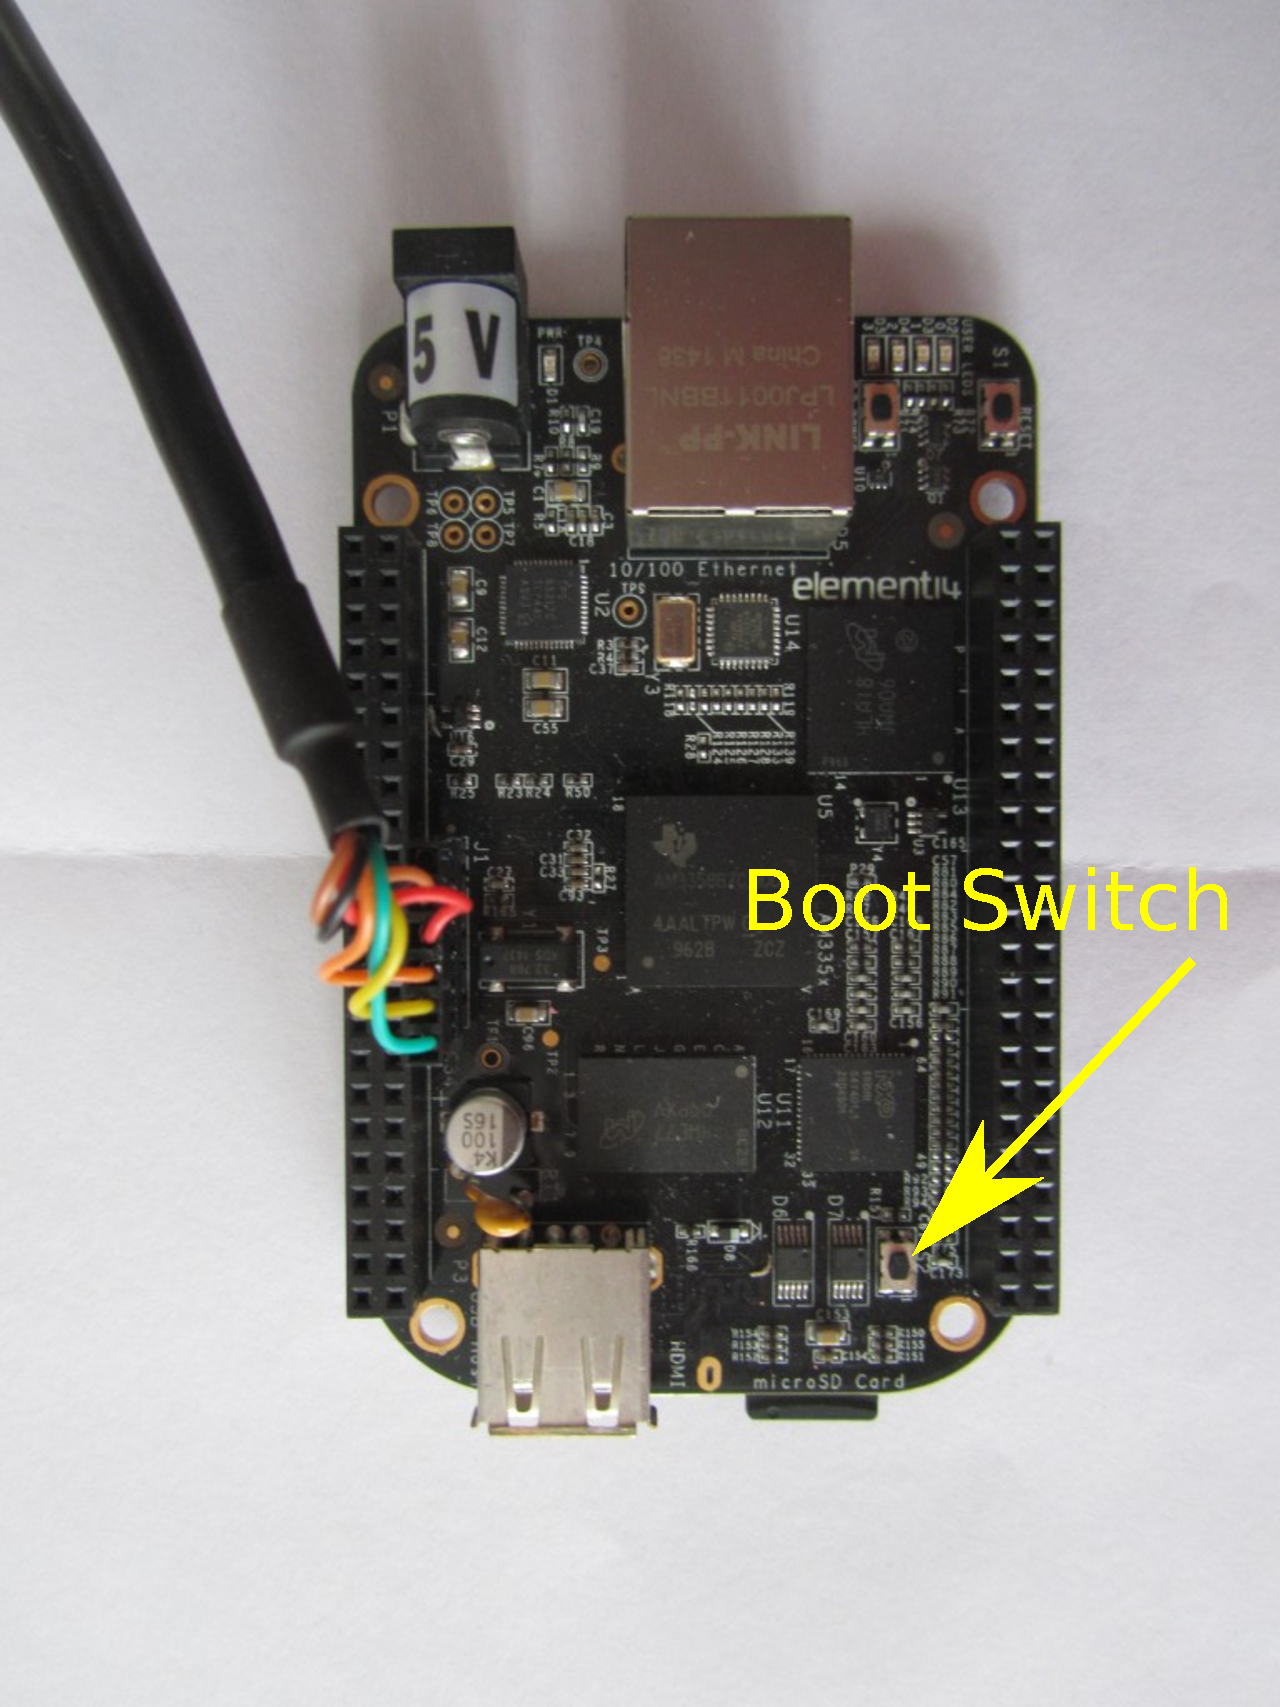
\includegraphics[width=0.75\textwidth]{boot-switch.pdf}
\end{column}
\end{columns} 
\end{frame}

\end{document}
